\begin{figure}[ht]
    \centering
    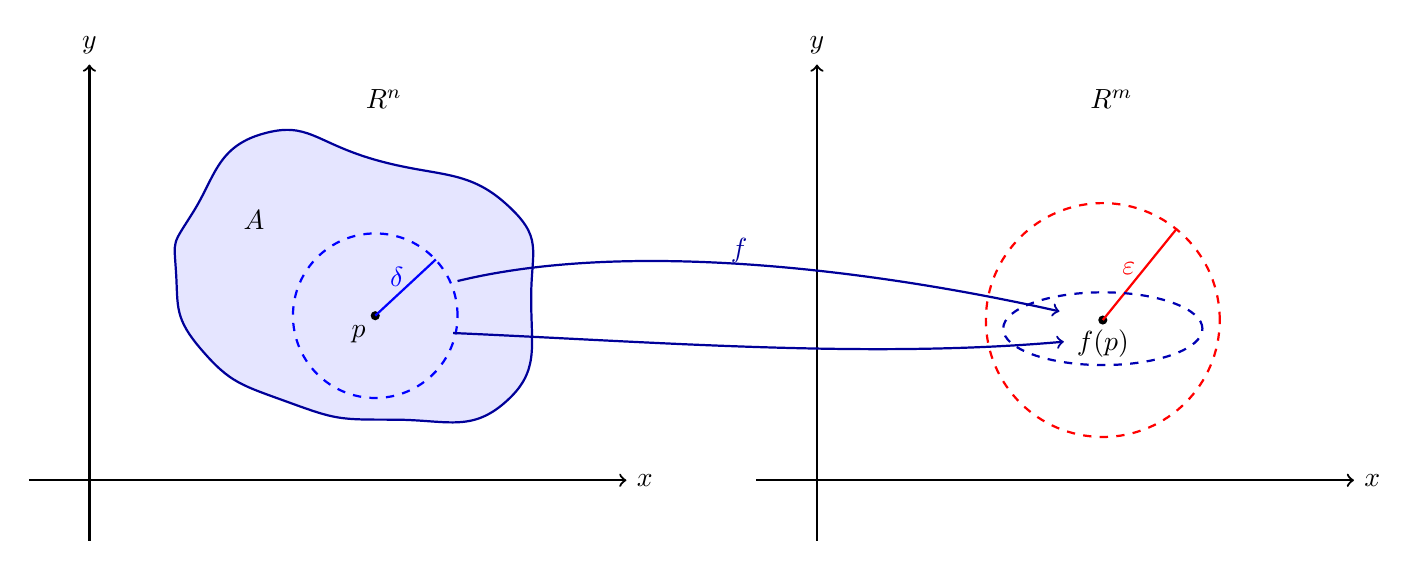
\begin{tikzpicture}[scale=1.1]

        %-------------------------
        % Plano da esquerda: R^n
        %-------------------------
        \draw[->, thick] (-0.7,0) -- (6.2,0) node[right] {$x$};
        \draw[->, thick] (0,-0.7) -- (0,4.8) node[above] {$y$};
        \node at (3.4,4.4) {$\mathbb{R}^n$};

        % Conjunto A em forma de ameba
        \draw[fill=blue!10, draw=blue!60!black, thick]
            plot[smooth cycle, tension=0.9] coordinates {
                (1.2,3.1) (2.0,4.0) (3.3,3.7) (4.8,3.2)
                (5.1,2.1) (4.8,0.9) (3.5,0.7) (2.3,0.9)
                (1.3,1.5) (1.0,2.4)
            };
        \node at (1.9,3.0) {$A$};

        % Ponto p
        \filldraw[black] (3.3,1.9) circle (1.3pt) node[below left] {$p$};

        % Bola delta
        \draw[blue, thick, dashed] (3.3,1.9) circle (0.95);

        % Raio delta
        \draw[blue, thick] (3.3,1.9) -- (4.0,2.55);
        \node[blue] at (3.55,2.35) {$\delta$};

        %-------------------------
        % Plano da direita: R^m
        %-------------------------
        \begin{scope}[xshift=8.4cm]
            \draw[->, thick] (-0.7,0) -- (6.2,0) node[right] {$x$};
            \draw[->, thick] (0,-0.7) -- (0,4.8) node[above] {$y$};
            \node at (3.4,4.4) {$\mathbb{R}^m$};

            % Ponto f(p)
            \filldraw[black] (3.3,1.85) circle (1.3pt) node[below] {$f(p)$};

            % Bola epsilon
            \draw[red, thick, dashed] (3.3,1.85) circle (1.35);

            % Raio epsilon
            \draw[red, thick] (3.3,1.85) -- (4.15,2.9);
            \node[red] at (3.6,2.45) {$\varepsilon$};

            % Imagem do B_delta(p) (esquemática)
            \draw[blue!70!black, thick, dashed] (3.3,1.75) ellipse (1.15 and 0.42);
        \end{scope}

        %-------------------------
        % Setas da aplicação
        %-------------------------
        \draw[->, thick, blue!60!black]
            (4.25,2.3) .. controls (6.3,2.8) and (9.2,2.4) .. (11.2,1.95);

        \draw[->, thick, blue!60!black]
            (4.2,1.7) .. controls (6.5,1.6) and (9.0,1.4) .. (11.25,1.6);

        \node[blue!60!black] at (7.5,2.65) {$f$};

    \end{tikzpicture}
    \caption{Ilustração da continuidade.}
\end{figure}